\section{Exploración Univariada}\label{univariada}




La población de Colombia se concentra en las áreas andinas y en la costa del Atlántico, donde se aprecian los núcleos demográficos de la sabana de Bogotá, conformado por Bogotá y Soacha, del valle de Aburrá, que comprende a Medellín, Bello e Itagüí, del Valle del Cauca, compuesto por Cali y Palmira. Lo mismo que las ciudades de la Costa Atlántica, Cartagena, Barranquilla y Santa Marta. Al igual que los centros demográficos de Bucaramanga y Cúcuta en la zona de los Santanderes, el Eje cafetero, Huila y Tolima.

En cuanto a su demografía, Colombia se caracteriza por ser el tercer país más poblado en Latinoamérica después de Brasil y México. Ha experimentado un rápido crecimiento poblacional como muchos países de la región, con un leve descenso en las últimas décadas. Alrededor de 3 millones de colombianos viven fuera del país a causa del conflicto armado. Sin embargo, gracias a mejoras económicas desde la década de los 2000, en los centros urbanos han mejorado los estándares de vida.

% Table created by stargazer v.5.2.2 by Marek Hlavac, Harvard University. E-mail: hlavac at fas.harvard.edu
% Date and time: lun., jul. 02, 2018 - 9:22:16 p. m.
\begin{table}[!htbp] \centering 
  \caption{Medidas estadísticas} 
  \label{stats} 
\begin{tabular}{@{\extracolsep{5pt}}lccccc} 
\\[-1.8ex]\hline 
\hline \\[-1.8ex] 
Statistic & \multicolumn{1}{c}{Mean} & \multicolumn{1}{c}{Median} & \multicolumn{1}{c}{St. Dev.} & \multicolumn{1}{c}{Min} & \multicolumn{1}{c}{Max} \\ 
\hline \\[-1.8ex] 
IDH & 0.802 & 0.804 & 0.042 & 0.691 & 0.879 \\ 
Poblacion.Cabecera & 1,196,730.000 & 717,197 & 1,982,287.000 & 13,090 & 10,070,801 \\ 
Poblacion.Resto & 360,590.300 & 268,111.5 & 331,887.600 & 21,926 & 1,428,858 \\ 
Poblacion.Total & 1,557,320.000 & 1,028,429 & 2,202,522.000 & 43,446 & 10,985,285 \\ 
\hline \\[-1.8ex] 
\end{tabular} 
\end{table} 




\begin{figure}[h]

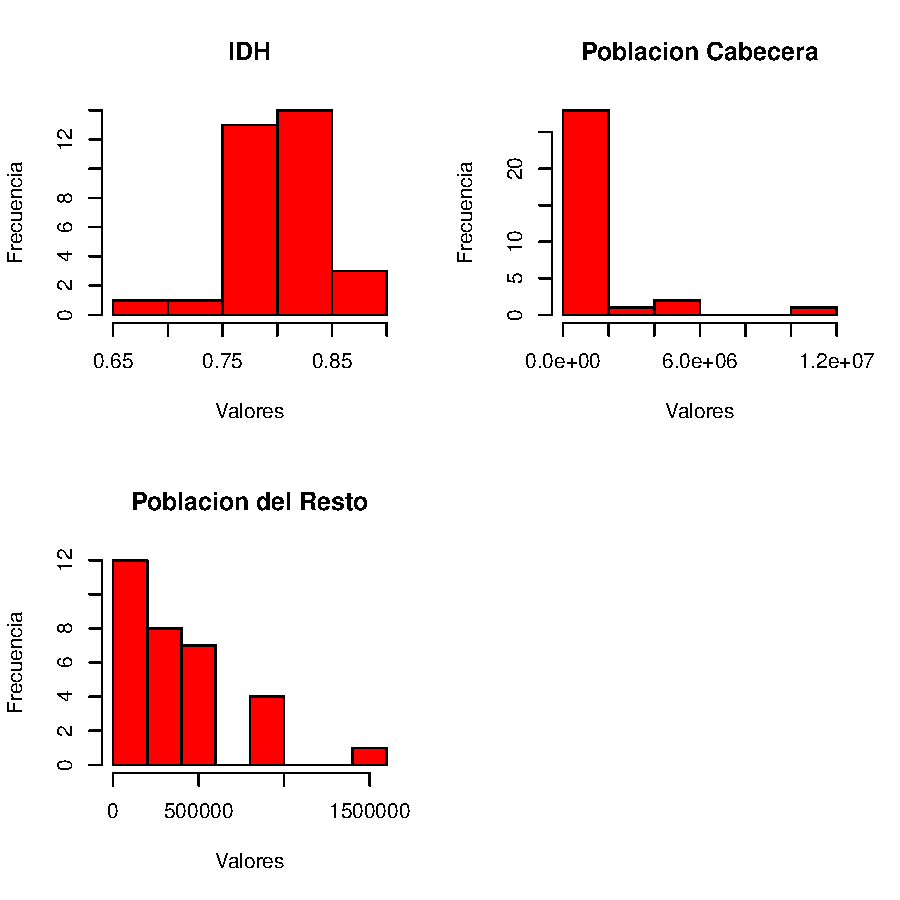
\includegraphics{univariada-hist}
\caption{Distribuci?n de Indicadores}
\label{hist}
\end{figure}

Si quieren normalizar dado el sesgo de las poblaciones, se tranforma con logaritmo en case 10 y quedaria asi:

\begin{figure}[h]
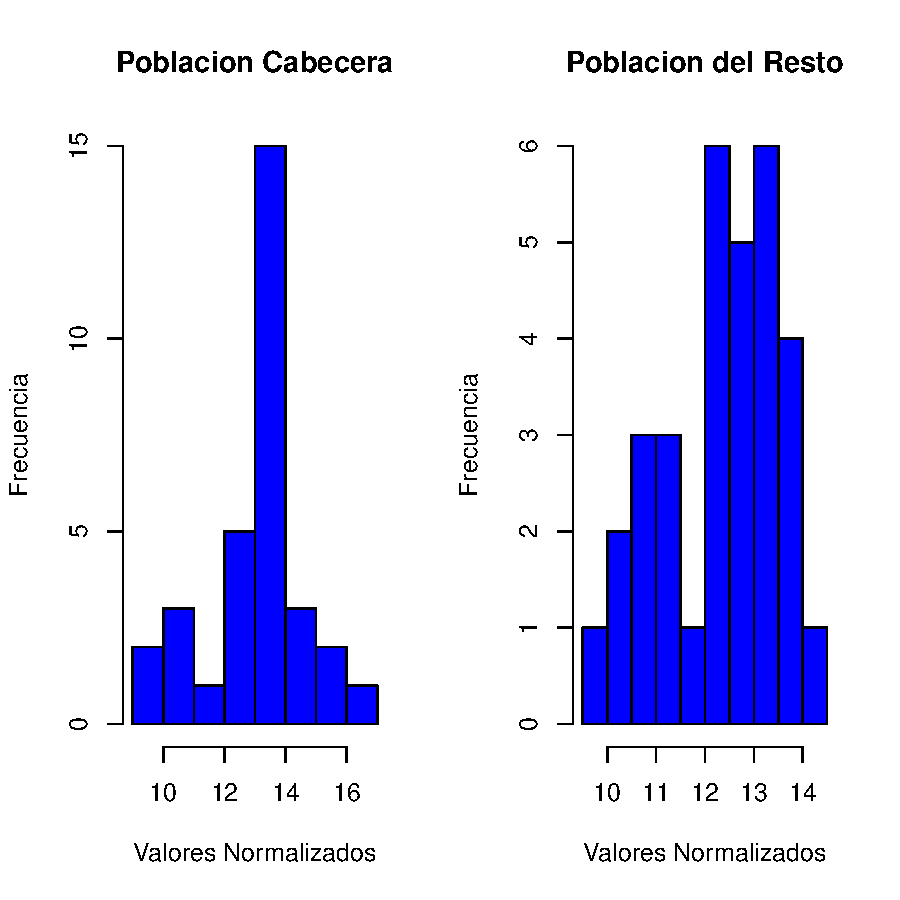
\includegraphics{univariada-hist1}
\caption{Distribuci?n de Indicadores de Poblaciones Normalizado}
\label{hist1}
\end{figure}

\endinput
